% \documentclass[handout]{beamer}
\documentclass{beamer}

\mode<presentation>
{
  \usetheme{default}
  \usefonttheme[onlymath]{serif}
  % \usetheme{Singapore}
  % \usetheme{Warsaw}
  % \usetheme{Malmoe}
  % \useinnertheme{circles}
  % \useoutertheme{infolines}
  % \useinnertheme{rounded}

  \setbeamercovered{transparent=5}
}

\usepackage[english]{babel}
\usepackage[latin1]{inputenc}
\usepackage{textpos,alltt,listings,multirow,ulem,siunitx}
\newcommand\hmmax{0}
\newcommand\bmmax{0}
\usepackage{bm}

% font definitions, try \usepackage{ae} instead of the following
% three lines if you don't like this look
\usepackage{mathptmx}
\usepackage[scaled=.90]{helvet}
% \usepackage{courier}
\usepackage[T1]{fontenc}
\usepackage{tikz}
\usetikzlibrary[shapes,shapes.arrows,arrows,shapes.misc,fit,positioning]

% \usepackage{pgfpages}
% \pgfpagesuselayout{4 on 1}[a4paper,landscape,border shrink=5mm]

\usepackage{JedMacros}

\title{Tightly Coupled Solvers, Loosely Coupled Software}
\subtitle{Multi-physics solvers and time integration in PETSc}

\author{Jed Brown, Emil Constantinescu, and Barry Smith}


% - Use the \inst command only if there are several affiliations.
% - Keep it simple, no one is interested in your street address.
\institute
{
  {Argonne National Laboratory} \\
}

\date{2011-11-02}

% This is only inserted into the PDF information catalog. Can be left
% out.
\subject{Talks}


% If you have a file called "university-logo-filename.xxx", where xxx
% is a graphic format that can be processed by latex or pdflatex,
% resp., then you can add a logo as follows:

% \pgfdeclareimage[height=0.5cm]{university-logo}{university-logo-filename}
% \logo{\pgfuseimage{university-logo}}



% Delete this, if you do not want the table of contents to pop up at
% the beginning of each subsection:
% \AtBeginSubsection[]
% {
% \begin{frame}<beamer>
%   \frametitle{Outline}
%   \tableofcontents[currentsection,currentsubsection]
% \end{frame}
% }

\AtBeginSection[]
{
  \begin{frame}<beamer>
    \frametitle{Outline}
    \tableofcontents[currentsection]
  \end{frame}
}

% If you wish to uncover everything in a step-wise fashion, uncomment
% the following command:

% \beamerdefaultoverlayspecification{<+->}

\begin{document}
\lstset{language=C}
\normalem

\begin{frame}
  \titlepage
\end{frame}

\begin{frame}{Multiphysics problems}
  \begin{block}{Examples}
    \begin{itemize}
    \item Saddle-point problems (\eg incompressibility, contact)
    \item Stiff waves (\eg low-Mach combustion)
    \item Mixed type (\eg radiation hydrodynamics, ALE free-surface flows)
    \item Multi-domain problems (\eg fluid-structure interaction)
    \item Full space PDE-constrained optimization
    \end{itemize}
  \end{block}
  \begin{block}{Software/algorithmic considerations}
    \begin{itemize}
    \item Separate groups develop different ``physics'' components
    \item Do not know a priori which methods will have good algorithmic properties
    \item Achieving high throughput is more complicated
    \item Multiple time and/or spatial scales
      \begin{itemize}
      \item Splitting methods are delicate, often not in asymptotic regime
      \item Strongest nonlinearities usually non-stiff: prefer explicit for TVD limiters/shocks
      \end{itemize}
    \end{itemize}
  \end{block}
\end{frame}

\begin{frame}{The Great Solver Schism: Monolithic or Split?}
  \begin{columns}
    \begin{column}{0.5\textwidth}
      \begin{block}{Monolithic}
        \begin{itemize}
        \item Direct solvers
        \item Coupled Schwarz
        \item Coupled Neumann-Neumann \\
          (need unassembled matrices)
        \item Coupled multigrid
        \item[X] Need to understand local spectral and compatibility properties of the coupled system
        \end{itemize}
      \end{block}
    \end{column}
    \begin{column}{0.5\textwidth}
      \begin{block}{Split}
        \begin{itemize}
        \item Physics-split Schwarz \\
          (based on relaxation)
        \item Physics-split Schur \\
          (based on factorization)
          \begin{itemize}
          \item  approximate commutators \\
            SIMPLE, PCD, LSC
          \item segregated smoothers
          \item Augmented Lagrangian
          \item ``parabolization'' for stiff waves
          \end{itemize}
        \item[X] Need to understand global coupling strengths
        \end{itemize}
      \end{block}
    \end{column}
  \end{columns}
  \begin{itemize}
  \item Preferred data structures depend on which method is used.
  \item Interplay with geometric multigrid.
  \end{itemize}
\end{frame}

\begin{frame}{Splitting for Multiphysics}
  \begin{equation*}
    \begin{bmatrix}
      A & B \\ C & D
    \end{bmatrix}
    \begin{bmatrix}
      x \\ y
    \end{bmatrix}
    =
    \begin{bmatrix}
      f \\ g
    \end{bmatrix}
  \end{equation*}
  \begin{itemize}\item Relaxation:
    \code{-pc\_fieldsplit\_type [additive,multiplicative,symmetric\_multiplicative]}
    \begin{equation*}
      \begin{bmatrix}
        A & \\  & D
      \end{bmatrix}^{-1} \qquad 
      \begin{bmatrix}
        A & \\ C & D
      \end{bmatrix}^{-1} \qquad
      \begin{bmatrix}
        A & \\  & \bm 1
      \end{bmatrix}^{-1}
      \left(
        \bm 1 -
        \begin{bmatrix}
          A & B \\ & \bm 1
        \end{bmatrix}
        \begin{bmatrix}
          A & \\ C & D
        \end{bmatrix}^{-1}
      \right)
    \end{equation*}
    \begin{itemize}
    \item Gauss-Seidel inspired, works when fields are loosely coupled
    \end{itemize}
  \item Factorization: \code{-pc\_fieldsplit\_type schur}
    \begin{align*}
      \begin{bmatrix}
        A & B \\ & S
      \end{bmatrix}^{-1}
      \begin{bmatrix}
        1 & \\ CA^{-1} & 1
      \end{bmatrix}^{-1}, \qquad
      S = D - C A^{-1} B
    \end{align*}
    \begin{itemize}
    \item robust (exact factorization), can often drop lower block
    \item how to precondition $S$ which is usually dense?
      \begin{itemize}
      \item interpret as differential operators, use approximate commutators
      \end{itemize}
    \end{itemize}
  \end{itemize}
\end{frame}

%\begin{frame}{Coupled approach to multiphysics}
  \begin{itemize}
  \item Smooth all components together
    \begin{itemize}
    \item Block SOR is the most popular
    \item Block ILU sometimes more robust (\eg transport/anisotropy)
    \item Vanka field-split smoothers or for saddle-point problems
    \item Distributive relaxation
    \end{itemize}
  \item Scaling between fields is critical
  \item Indefiniteness
    \begin{itemize}
    \item Make smoothers and interpolants respect inf-sup condition
    \item Difficult to handle anisotropy
    \item Exotic interpolants for Helmholtz
    \end{itemize}
  \item Transport
    \begin{itemize}
    \item Define smoother in terms of first-order upwind discretization ($h$-ellipticity)
    \item Evaluate residuals using high-order discretization
    \item Use Schur field-split: ``parabolize'' at top level or for smoother on levels
    \end{itemize}
  \item Multigrid inside field-split or field-split inside multigrid
  \item Open research area, hard to write modular software
  \end{itemize}
\end{frame}

\begin{frame}[shrink=10]{``Physics-based'' preconditioners (semi-implicit method)}
  \begin{block}{Shallow water with stiff gravity wave}
    $h$ is hydrostatic pressure, $u$ is velocity, $\sqrt{gh}$ is fast wave speed
    \begin{gather*}
      h_t - (uh)_x = 0 \\
      (uh)_t + (u^2h + \half gh^2)_x = 0
    \end{gather*}
  \end{block}
  \vspace{-3em}
  \begin{block}{Semi-implicit method}
    Suppress spatial discretization, discretize in time, implicitly for the terms contributing to the gravity wave
    \begin{gather*}
      \frac{h^{n+1} - h^n}{\Delta t} + (uh)_x^{n+1} = 0 \\
      \frac{(uh)^{n+1} - (uh)^{n}}{\Delta t} + (u^2h)_x^{n} + g(h^n h^{n+1})_x = 0
    \end{gather*}

    Rearrange, eliminating $(uh)^{n+1}$
    \[ \frac{h^{n+1} - h^n}{\Delta t} - \Delta t(gh^n h_x^{n+1})_x = -S_x^n \]
  \end{block}
\end{frame}

\begin{frame}[shrink=1]{Delta form}
  \begin{itemize}
  \item Preconditioner should work like the Newton step: $-F(x) \mapsto \delta x$
  \item Recast semi-implicit method in delta form
    \[ \frac{\delta h}{\Delta t} + (\delta uh)_x = -F_0, \quad \frac{\delta uh}{\Delta t} + g h^n (\delta h)_x = -F_1,
    \quad \widehat{J} =
    \begin{pmatrix}
      \frac{1}{\Delta t} & \div \\
      g h^n \nabla & \frac{1}{\Delta t}
    \end{pmatrix}
    \]
  \item Eliminate $\delta uh$
    \[ \frac{\delta h}{\Delta t} - \Delta t(gh^n (\delta h)_x)_x = -F_0 + (\Delta t F_1)_x,
    \quad S \sim \frac{1}{\Delta t} - g \Delta t \div h^n \nabla
    \]
  \item Solve for $\delta h$, then evaluate
    \[ \delta uh = - \Delta t \big[ gh^n (\delta h)_x - F_1 \big] \]
  \item Fully implicit solver
    \begin{itemize}
    \item Is nonlinearly consistent (no splitting error), can be high-order in time
    \item Uses existing code when a semi-implicit method has been implemented
    \item Allows efficient bifurcation analysis, steady-state analysis
    \end{itemize}
  \end{itemize}
\end{frame}


\section{Coupling software}
\begin{frame}{Multi-physics coupling in PETSc}
  \begin{columns}
    \begin{column}{0.5\textwidth}
      \tikzstyle{cloud} = [draw, ellipse,fill=red!20, node distance=3cm, minimum height=2em]
      \tikzstyle{block} = [rectangle, draw, fill=blue!20, text width=5em, text centered, rounded corners, minimum height=2em]
      \begin{tikzpicture}
        \node [cloud] (momentum) {Momentum};
        \node [cloud, right of=momentum] (pressure) {Pressure};
        \node<2-> [block, opacity=0.5, fit=(momentum)(pressure), text opacity=0.8] (stokes) {Stokes};
        \node<3-> [cloud, below=2em of momentum] (energy) {Energy};
        \node<3-> [cloud, below=2em of pressure] (geometry) {Geometry};
        \node<4-> [block, opacity=0.4, fit=(stokes)(momentum)(pressure)(energy)(geometry), text opacity=0.8, text height=4em] (ice) {Ice};
        \node<5-> [block, below=2em of ice, minimum width=16em] (bl) {{Boundary \nolinebreak Layer}};
        \node<5-> [block, below=2em of bl, minimum width=16em] (ocean) {Ocean};
        % ]
      \end{tikzpicture}
    \end{column}
    \begin{column}{0.5\textwidth}
      \begin{itemize}
      \item package each ``physics'' independently
      \item solve single-physics and coupled problems
      \item semi-implicit and fully implicit
      \item reuse residual and Jacobian evaluation unmodified
      \item direct solvers, fieldsplit inside multigrid, multigrid inside fieldsplit without recompilation
      \item use the best possible matrix format for each physics \\ (e.g. symmetric block size 3)
      \item matrix-free anywhere
      \item multiple levels of nesting
      \end{itemize}
    \end{column}
  \end{columns}
\end{frame}

\begin{frame}
  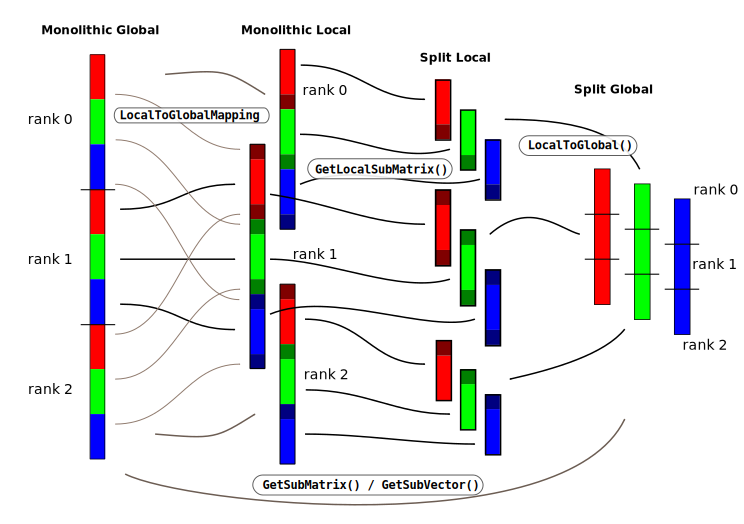
\includegraphics[width=\textwidth]{figures/PETSc/LocalSpaces} \\[-.5em]
  Work in Split Local space, matrix data structures reside in any space.
\end{frame}

%\begin{frame}[fragile]{\cfunc|MatGetLocalSubMatrix| spaces}
  \begin{itemize}
  \item Newton method for $F(x) = 0$ solves
    \begin{gather*}
      J(x) \delta x = - F(x) \\
      J = \begin{pmatrix}
      J_{aa} & J_{ab} & J_{ac} \\
      J_{ba} & J_{bb} & J_{bc} \\
      J_{ca} & J_{cb} & J_{cc}
    \end{pmatrix} .
    \end{gather*}
  \item Conceptually, there are three spaces in parallel
    \begin{itemize}
    \item[$V$] Globally assembled space
    \item[$V_i$] Global space for a single physics $i$
    \item[$\bar V_i$] Local space (with ghosts) for a single physcs $i$
    \item[$\bar V$] $\prod_i \bar V_i$ Concatenation of all single-physics local spaces
    \end{itemize}
  \item Different components need different relationships
    \begin{itemize}
    \item[$V_i \to V$] field-split
    \item[$\bar V \to V$] coupled Neumann domain decomposition methods
    \item[$\bar V_i$] natural language for modular residual evaluation and assembly
    \end{itemize}
  \end{itemize}
\end{frame}

\begin{frame}[fragile]{\cfunc|MatGetLocalSubMatrix| spaces}
  \begin{block}{Spaces}
    \begin{itemize}
    \item[$V$] Globally assembled space
    \item[$V_i$] Global space for a single physics $i$
    \item[$\bar V_i$] Local space (with ghosts) for a single physcs $i$
    \item[$\bar V$] $\prod_i \bar V_i$ Concatenation of all
      single-physics local spaces
    \end{itemize}
  \end{block}
  \begin{itemize}
  \item Multiple physics $x = [x_a,x_b,x_c]$
  \item[$I_i$] Map indices from $V_i$ to $V$.
  \item[$R_i$] Global physics restriction $R_i : V \to V_i$
    \[ R_i x = x[I_i] = x_i \]
  \item[$\bar I_i$] Map indices from $\bar V_i$ to $V_i$
  \item[$\bar R_i$] Extract local single-physics part from global single-physics
    \[ \bar R_i x_i = x_i[\bar I_i] = \bar x_i \]
  \item[$\tilde I_i$] Map indices from $\bar V_i$ to $\bar V$
  \end{itemize}
\end{frame}

\begin{frame}[fragile]{\cfunc|MatGetLocalSubMatrix| spaces}
\begin{itemize}
    \item Globally assembled coupled matrix in terms of assembled single-physics blocks
    \[ J = \sum_{ij} R_i^T J_{ij} R_j \]
    \begin{itemize}
    \item Language of Schwarz and fieldsplit
    \end{itemize}
  \item Assembled single-physics blocks in terms of local single-physics matrices
    \[ J_{ij} = \bar R_i^T \bar J_{ij} \bar R_j \]
    \begin{itemize}
    \item Language of assembly and Neumann/FETI domain decomposition
    \item \cfunc|MatSetValuesLocal|
    \end{itemize}
  \end{itemize}
\end{frame}

\begin{frame}
  \alert{\texttt{MatGetLocalSubMatrix(Mat A,IS rows,IS cols,Mat *B);}}
  \begin{itemize}
  \item Primarily for assembly
    \begin{itemize}
    \item \texttt{B} is not guaranteed to implement \texttt{MatMult}
    \item The communicator for \texttt{B} is not specified, \\
      only safe to use non-collective ops (unless you check)
    \end{itemize}
  \item \texttt{IS} represents an index set, includes a block size and communicator
  \item \texttt{MatSetValuesBlockedLocal()} is implemented
  \item MatNest returns nested submatrix, no-copy
  \item No-copy for Neumann-Neumann formats \\ (unassembled across procs, e.g. BDDC, FETI-DP)
  \item Most other matrices return a lightweight proxy \texttt{Mat}
    \begin{itemize}
    \item \texttt{COMM\_SELF}
    \item Values not copied, does not implement \texttt{MatMult}
    \item Translates indices to the language of the parent matrix
    \item Multiple levels of nesting are flattened
    \end{itemize}
  \end{itemize}
\end{frame}


\section{Applications}
%\newcommand{\colorA}[1]{{\color{red} #1}}
\newcommand{\colorB}[1]{{\color{green!60!black} #1}}
\newcommand{\colorC}[1]{{\color{blue} #1}}
\newcommand{\colorD}[1]{{\color{magenta!70!black} #1}}
\newcommand{\colorE}[1]{{\color{cyan!70!black} #1}}
\newcommand{\colorF}[1]{{\color{yellow!60!black} #1}}
\newcommand{\colorG}[1]{{\color{red!50!white} #1}}

\begin{frame}{ALE form}
  After discretization in time ($\alpha \propto 1/\Delta t$) we have a Jacobian
  \begin{equation*}
    \begin{bmatrix}
      \colorA{A_{II}} & \colorA{A_{I\Gamma}}             &                       &                             &                     &   \\
      & \colorB{\alpha M_{\Gamma\Gamma}} &                       & \colorB{- N_{\Gamma\Gamma}} &                       &  \\
      \colorG{G_{II}}      & \colorG{G_{\Gamma I}} & \colorC{B_{II}}       & \colorC{B_{I\Gamma}}        & \colorC{C_{I}^T}    & \colorD{D_I} \\
      \colorG{G_{I\Gamma}} &        \colorG{G_{\Gamma\Gamma}}                          & \colorC{B_{\Gamma I}} & \colorC{B_{\Gamma\Gamma}}   & \colorC{C_{\Gamma}^T} & \colorD{D_\Gamma} \\
      \colorG{G_{Ip}}        &  \colorG{G_{\Gamma p}}                                & \colorC{C_{I}}        & \colorC{C_{\Gamma}}         &                   & \\
      \colorE{\alpha E_I}    & \colorE{\alpha E_\Gamma} & \colorE{F_I} & \colorE{F_\Gamma} & & \colorF{\alpha M_\Theta + J}
    \end{bmatrix}
    \begin{bmatrix}
      x_I \\ x_\Gamma \\ u_I \\ u_\Gamma \\ p \\ \Theta
    \end{bmatrix}
  \end{equation*}
  \begin{itemize}
  \item \colorA{mesh motion equations (Laplace-Beltrami or pseudo-elasticity)}
  \item \colorB{$(\dot{\bm x} - \bm u)\cdot \bm n = \text{accumulution}$}
  \item \colorG{``just'' geometry}
  \item \colorC{Stokes problem}
  \item \colorD{temperature dependence of rheology}
  \item \colorE{convective terms and strain heating in heat transport}
  \item \colorF{thermal advection-diffusion}
  \end{itemize}
\end{frame}

\subsection{Ice Flow}
\newcommand\smallterm[1]{{\color{gray} #1}}
\begin{frame}{Conservative two-phase formulation}
  Find momentum density $\rho\uu$, pressure $p$, and total energy density $E$:
  \begin{gather*}
    (\rho\uu)_t + \div (\smallterm{\rho\uu\otimes\uu} - \eta D\uu_i + p\bm 1) - \rho \bm g = 0 \\
    \rho_t + \div \rho\uu = 0 \\
    E_t + \div \big((E+p)\uu - k_T\nabla T - k_\omega\nabla\omega \big) - \eta D\uu_i\tcolon D\uu_i - \smallterm{\rho\uu\cdot\bm g} = 0
  \end{gather*}
\begin{itemize}
\item Solve for density $\rho$, ice velocity $\uu_i$, temperature $T$, and melt fraction $\omega$ using constitutive relations.
  \begin{itemize}
  \item Simplified constitutive relations can be solved explicitly.
  \item Temperature, moisture, and strain-rate dependent rheology $\eta$.
  \item High order FEM, typically $Q_3$ momentum \& energy, SUPG (yuck).
  \end{itemize}
\item DAEs solved implicitly after semidiscretizing in space.
\item Preconditioning using nested fieldsplit
\end{itemize}
\end{frame}
\begin{frame}{Relative effect of the blocks}
  \begin{equation*}\label{eq:vhtblock}
    J =
    \begin{pmatrix}
      J_{uu} & J_{up} & J_{uE} \\
      J_{pu} & 0 & 0 \\
      J_{Eu} & J_{Ep} & J_{EE}
    \end{pmatrix} .
  \end{equation*}
  \begin{itemize}
  \item[$J_{uu}$] Viscous/momentum terms, nearly symmetric, variable coefficionts, anisotropy from Newton.
  \item[$J_{up}$] Weak pressure gradient, viscosity dependence on pressure (small), gravitational contribution (pressure-induced density variation).
    Large, nearly balanced by gravitational forcing.
  \item[$J_{uE}$] Viscous dependence on energy, very nonlinear, not very large.
  \item[$J_{pu}$] Divergence (mass conservation), nearly equal to $J_{up}^T$.
  \item[$J_{Eu}$] Sensitivity of energy on momentum, mostly advective transport.
    Large in boundary layers with large thermal/moisture gradients.
  \item[$J_{Ep}$] Thermal/moisture diffusion due to pressure-melting, $\uu \cdot \nabla$.
  \item[$J_{EE}$] Advection-diffusion for energy, very nonlinear at small regularization.
    Advection-dominated except in boundary layers and stagnant ice, often balanced in vertical.
  \end{itemize}
\end{frame}

\begin{frame}{How much nesting?}
  \begin{columns}
    \begin{column}{0.5\textwidth}
      \begin{equation*}
        P_1 =
        \begin{pmatrix}
          J_{uu} & J_{up} & J_{uE} \\
          0 & B_{pp} & 0 \\
          0 & 0 & J_{EE} \\
        \end{pmatrix}
      \end{equation*}
      \begin{itemize}
      \item $B_{pp}$ is a mass matrix in the pressure space weighted by inverse of kinematic viscosity.
      \item Elman, Mihajlovi\'c, Wathen, JCP 2011 for non-dimensional isoviscous Boussinesq.
      \item Works well for non-dimensional problems on the cube, not for realistic parameters.
      \end{itemize}
    \end{column}
    \begin{column}{0.5\textwidth}
      \begin{equation*}
        P =
        \begin{bmatrix}
          \begin{pmatrix}
            J_{uu} & J_{up} \\
            J_{pu} & 0
          \end{pmatrix} & \\
          \begin{pmatrix}
            J_{Eu} & J_{Ep}
          \end{pmatrix}
          & J_{EE}
        \end{bmatrix}
      \end{equation*}
      \begin{itemize}
      \item Inexact inner solve using upper-triangular with $B_{pp}$ for Schur.
      \item Another level of nesting.
      \item GCR tolerant of inexact inner solves.
      \item Outer converges in 1 or 2 iterations.
      \end{itemize}
    \end{column}
  \end{columns}
  \begin{itemize}
  \item Low-order preconditioning full-accuracy unassembled high order operator.
  \item Build these on command line with PETSc \cverb|PCFieldSplit|.
  \end{itemize}
\end{frame}


\subsection{Geodynamics}
\begin{frame}[shrink=5]{The Drunken Seaman instability}
  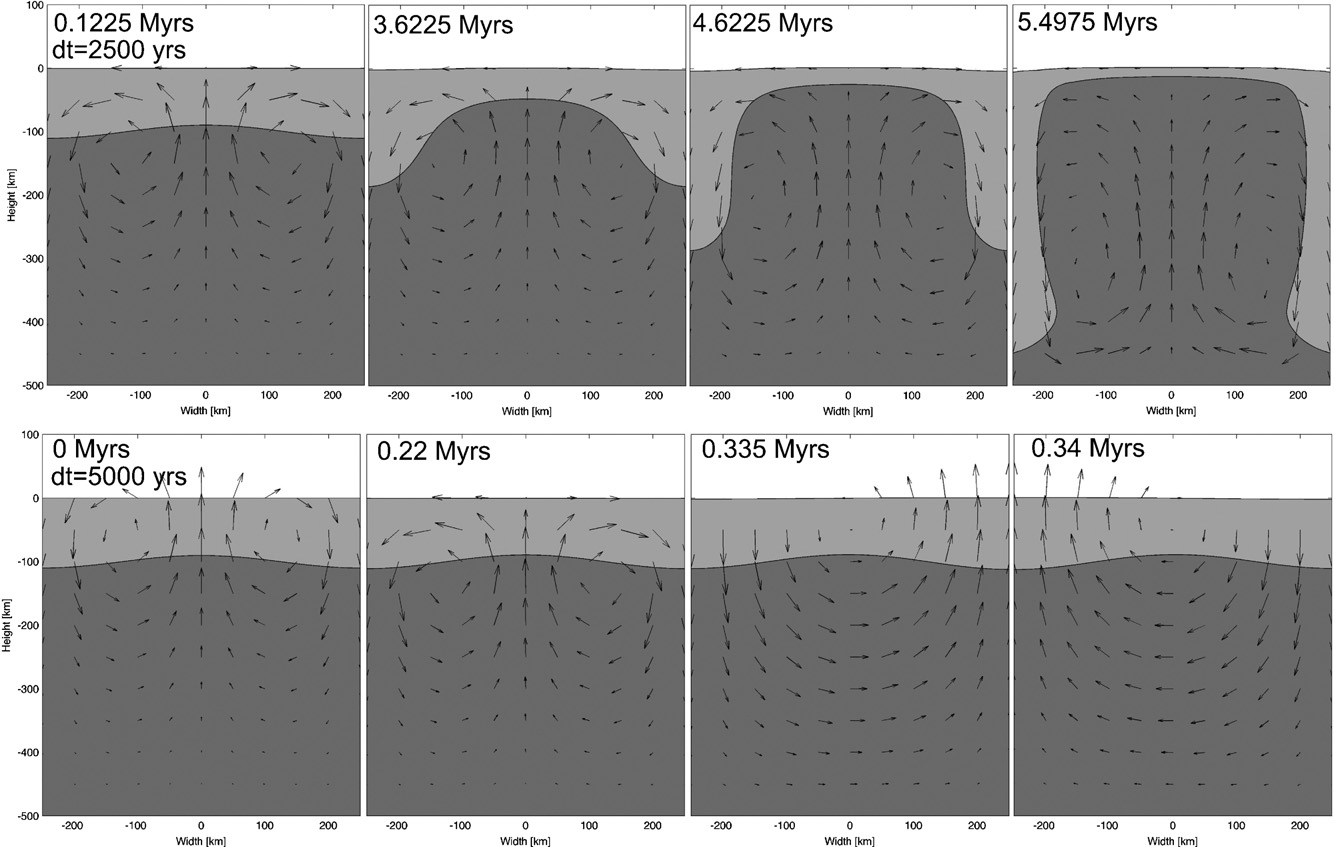
\includegraphics[width=0.9\textwidth]{figures/DrunkenSeaman} \\
  \begin{columns}
    \begin{column}{0.8\textwidth}
      \begin{itemize}
      \item Subduction and mantle convection with a free surface.
      \item Free surface critical to long-term dynamics \\
        (\eg mountain range formation)
      \item Advective 0.01 CFL for stability.
      \item Semi-implicit helps: Kaus, M\"uhlhaus, and May, 2010
      \end{itemize}
    \end{column}
    \begin{column}{0.2\textwidth}
      
\includegraphics[width=0.9\textwidth]{figures/DrunkenSeamanBottle}
    \end{column}
  \end{columns}
\end{frame}

\begin{frame}[fragile]{Fully implicit free surface}
  \begin{itemize}
  \item Velocity $u$, pressure $p$, Lagrangian/ALE coordinates $x$.
    \begin{equation*}
      J =
      \begin{pmatrix}
        J_{uu} & J_{up} & J_{ux} \\
        J_{pu} & 0 & J_{ux} \\
        J_{xu} & 0 & J_{xx}
      \end{pmatrix} .
    \end{equation*}
  \item Precondition with
    \begin{align*}
      P &=
      \begin{bmatrix}
        \begin{pmatrix}
          J_{uu} & J_{up} \\
          J_{pu} & 0
        \end{pmatrix} & \\
        \begin{pmatrix}
          J_{xu} & 0
        \end{pmatrix}
        & J_{xx}
      \end{bmatrix} &
      P_{\text{Stokes}} &=
      \begin{pmatrix}
        J_{uu} & 0 \\
        J_{pu} & B_{pp}
      \end{pmatrix}
    \end{align*}
  \item {\scriptsize
\begin{verbatim}
-dm_mat_type nest -pc_type fieldsplit
-fieldsplit_stokes_pc_type fieldsplit
-fieldsplit_stokes_pc_fieldsplit_type schur
-fieldsplit_stokes_pc_fieldsplit_schur_factorization_type lower
-fieldsplit_stokes_fieldsplit_u_pc_type mg
\end{verbatim}
}
\item {\scriptsize
\begin{verbatim}
-dm_mat_type aij -pc_type lu -pc_factor_mat_solver_package mumps
\end{verbatim}
}
  \end{itemize}
\end{frame}


\section{Implicit-Explicit time integration}
\begin{frame}[shrink=5]{IMEX time integration in PETSc}
  \begin{itemize}
  \item Additive Runge-Kutta IMEX methods
    \begin{gather*}
      G(t,x,\dot x) = F(t,x) \\
      J_\alpha = \alpha G_{\dot x} + G_x
    \end{gather*}
    \begin{itemize}
    \item User provides:
      \begin{itemize}
      \item \texttt{FormRHSFunction(ts,$t$,$x$,$F$,void *ctx);}
      \item \texttt{FormIFunction(ts,$t$,$x$,$\dot x$,$G$,void *ctx);}
      \item \texttt{FormIJacobian(ts,$t$,$x$,$\dot x$,$\alpha$,$J$,$J_{p}$,mstr,void *ctx);}
      \end{itemize}
    \item L-stable DIRK for stiff part $G$
    \item Choice of explicit method, \eg SSP
    \item Orders 2 through 5, embedded error estimates
    \item Dense output, hot starts for Newton
    \item More accurate methods if $G$ is linear, also Rosenbrock-W
    \item Can use preconditioner from classical ``semi-implicit'' methods
    \item Extensible adaptive controllers, can change order within a family
    \item Easy to register new methods: \code{TSARKIMEXRegister()}
    \end{itemize}
  \item Eliminate many interface quirks
  \item Single step interface so user can have own time loop
  \end{itemize}
\end{frame}


\section{Variational Inequalities}
\begin{frame}{Variational Inequalities}
  \begin{itemize}
  \item Supports inequality and box constraints on solution variables.
  \item Solution methods
    \begin{itemize}
    \item Semismooth Newton
      \begin{itemize}
      \item reformulate problem as a non-smooth system, Newton on subdifferential
      \item Newton step solves diagonally perturbed systems
      \end{itemize}
    \item Active set
      \begin{itemize}
      \item similar linear algebra to solving PDE
      \item sometimes slower convergence or ``bouncing''
      \end{itemize}
    \end{itemize}
  \item composes with multigrid and field-split
  \item demonstrated optimality for phase-field problems with millions of degrees of freedom
  \end{itemize}
\end{frame}


\begin{frame}{Outlook}
  \begin{itemize}
  \item Unified algebraic interface for monolithic and nested formats
  \item Improves software modularity, but still manages stiff coupling
  \item Block and symmetric formats
  \item Multigrid inside or outside field splits
  \item Can use IMEX methods $g(t,x,\dot x) = f(t,x)$
  \item Variational inequalities
  \item Still to do:
    \begin{itemize}
    \item Better preallocation for off-diagonal blocks
    \item Nonlinear solvers for IMEX systems with structure
    \item General/nonsymmetric pivoting in fieldsplit
    \item Change of variables for fieldsplit \\ (e.g. low-Mach Euler in conservative variables)
    \end{itemize}
  \end{itemize}
\end{frame}

\end{document}
